\documentclass[aspectratio=169]{beamer}
\usetheme{default}
\usecolortheme{dove}
\usepackage{booktabs,graphicx}
\graphicspath{{../results/figures/}}
\setbeamertemplate{navigation symbols}{}
\title{Which Operating Conditions Are Worth Simulating?}
\subtitle{Value-guided data acquisition for SCED under topology shift}
\author{Anonymous}
\date{PhD Interview, 25 August 2026}
\begin{document}

\begin{frame}{1. Problem: simulation labels have unequal value}
\begin{columns}[T]
\column{.57\textwidth}
\begin{itemize}
\item A learned surrogate predicts secure generator dispatch.
\item The grid changes: line 8 is removed from a six-bus network.
\item Target-topology SCED labels have a limited budget.
\end{itemize}
\vspace{.5em}
\alert{Question:} which operating conditions should we simulate so that each new label improves the downstream decision?
\column{.39\textwidth}
\begin{block}{Structural shift}
Source: all 10 lines\\[.5em]
Target: \alert{line 8 removed}
\end{block}
\vspace{.5em}
Matched diagnostic:\\
$+0.077$ MW MAE\\
$+0.55$ mean regret
\end{columns}
\end{frame}

\begin{frame}{2. Gap: prediction error is not operational value}
\begin{itemize}
\item Coverage finds unusual inputs; uncertainty finds model disagreement.
\item Neither explicitly asks whether an error matters for network constraints.
\item Dispatch MAE can rank models differently from repair burden and cost regret.
\end{itemize}
\begin{block}{Testable idea}
Weight uncertainty by predicted proximity to a base-case or contingency line limit---without observing the hidden SCED label.
\end{block}
\end{frame}

\begin{frame}{3. Method: one fair, leakage-controlled loop}
\centering
\Large 220 source labels $\rightarrow$ 5-MLP ensemble $\rightarrow$ target pool\\[.5em]
\normalsize
\begin{tabular}{llll}
Random & Diversity & Uncertainty & $\tilde u(1+\tilde c)$\\
\end{tabular}
\vspace{1em}
\begin{itemize}
\item 160 candidates; 12 shared initial labels; four batches of 12.
\item Same model, seeds, repair, label budgets, and untouched 80-case test set.
\item Evaluate raw security feasibility, $\ell_1$ repair, and repaired-cost regret.
\end{itemize}
\end{frame}

\begin{frame}{4. Result: uncertainty wins; weighting can hurt}
\begin{columns}[T]
\column{.58\textwidth}
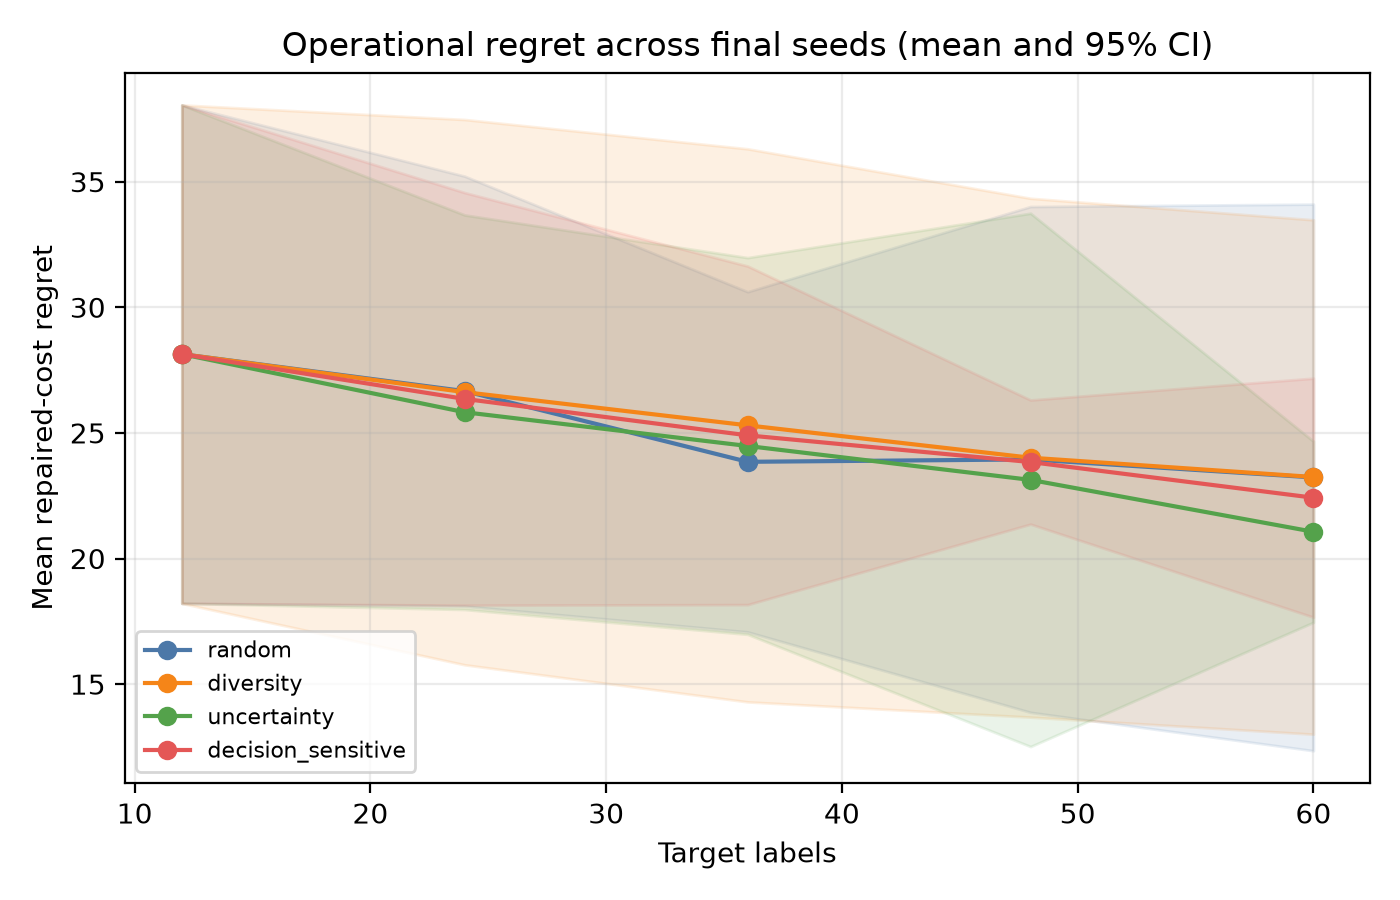
\includegraphics[width=\linewidth]{regret_vs_labels.png}
\column{.39\textwidth}
At 60 labels (three-seed means):
\begin{center}
\begin{tabular}{lrr}\toprule
Method & MAE & Regret\\\midrule
Random&1.582&23.23\\
Diversity&1.504&23.24\\
Uncertainty&\textbf{1.387}&\textbf{21.06}\\
Weighted&1.425&22.42\\\bottomrule
\end{tabular}
\end{center}
\small The decision-sensitive heuristic does not beat uncertainty; one case is worse by 54.253 regret units.
\end{columns}
\end{frame}

\begin{frame}{5. PhD extension: from heuristic to value of information}
\begin{enumerate}
\item Calibrate uncertainty and operational criticality on validation data.
\item Estimate expected repair or regret reduction before querying a label.
\item Scale to multiple outages, larger grids, AC-OPF, and dynamic simulators.
\item Use real measurement correlations to construct credible scenarios.
\end{enumerate}
\begin{block}{Take-away}
Decision-aware acquisition is worth testing, but it succeeds only when its proxy for downstream value is reliable.
\end{block}
\end{frame}
\end{document}
